\documentclass{beamer}
\usepackage{graphicx} % Za nalaganje slik
\usepackage[slovene]{babel}
\title{Predstavitev naloge}
\author{Vaše ime}
\date{2024}

\begin{document}

% 1. Prosojnica: Uvodna prosojnica
\frame{\titlepage}

% 2. Prosojnica: Kazalo
\begin{frame}
\frametitle{Kazalo}
    \tableofcontents
\end{frame}

% 3. Prosojnica: Predstavitev grafa P(t)
\begin{frame}
\frametitle{Graf P(t)}
    Na naslednjem grafu je prikazan potek moči $P(t)$ v odvisnosti od časa $t$.
    \begin{figure}
        \centering
        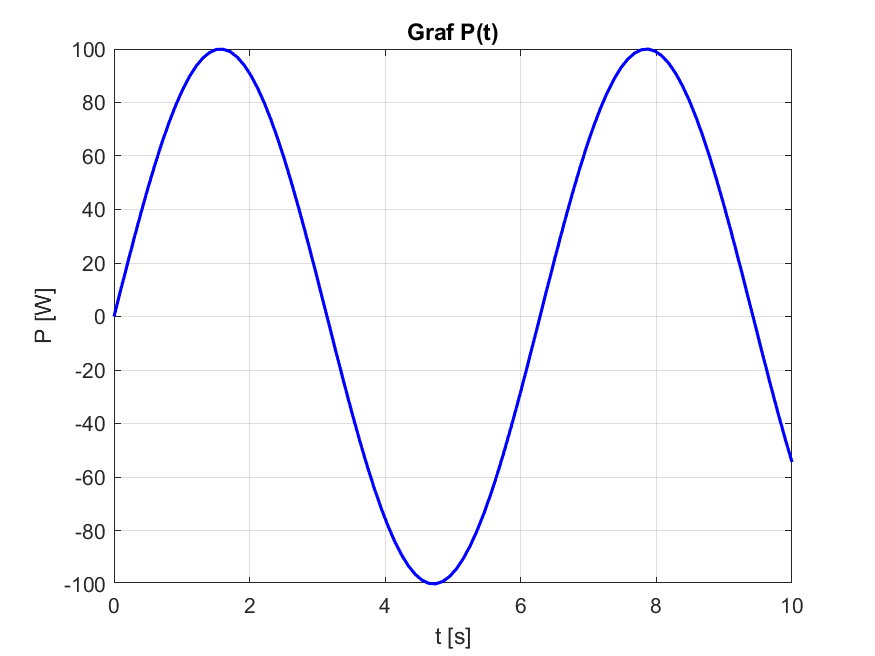
\includegraphics[width=0.8\textwidth]{graf.png} % Poskrbite, da je graf.png v isti mapi kot .tex datoteka
        \caption{Graf funkcije P(t)}
    \end{figure}
\end{frame}

\end{document}
